\clearpage
\section{Lösungskonzept}\label{sec:Loesungskonzept}
Zur Messung und Auswertung der Mesh-Netzwerke dient ein Testframework wie es in Abbildung \ref{fig:KonzeptschemaTestframework} schematisch dargestellt ist.

\begin{figure}[H]
	\centering
	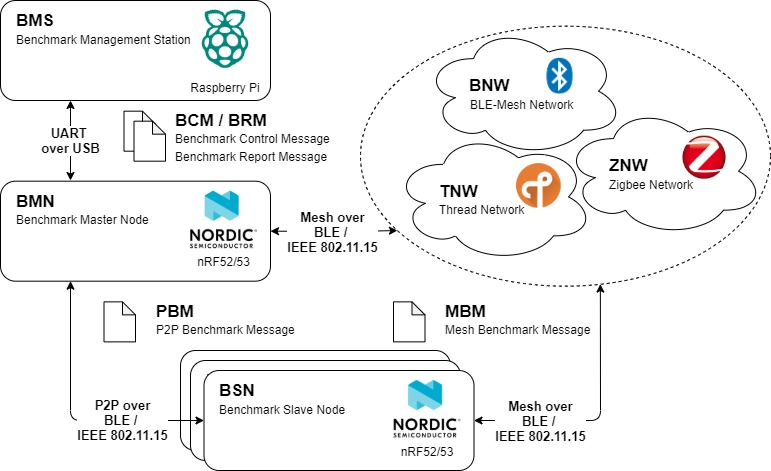
\includegraphics[width=1.0\textwidth]{Konzept_Testframework.jpg}
	\caption{Konzeptschema Testframework}\label{fig:KonzeptschemaTestframework}
\end{figure}


Das Testframework besteht aus folgenden physikalisch getrennten Teilsystemen:

\begin{itemize}
	\item \textbf{BMS} Benchmark Management Station \\ 
	Dient zur Verwaltung und Konfiguration des Testframeworks. Beinhaltet einen Webserver um dem Endanwender die Bedienung zu ermöglichen. Realisiert wird die BMS durch einen \textit{Raspberry Pi 4 Model B}. Als Webserver wird das Python-Framework \textit{Django} eingesetzt. 
	\item \textbf{BMN} Benchmark Master Node \\ 
	Dient als Zugangspunkt der BMS für die im Testframework gefahrenen Tests und lässt sich über eine Serielle Schnittstelle ansprechen. In der Aufgabenstellung \ref{app:Aufgabenstellung} wird der BMN als Master bezeichnet. Realisiert wird der BMN über einen nRF52840 oder nRF5340 von \textit{Nordic}. 
	\item \textbf{BSN} Benchmark Slave Node \\ 
	Dient als Zugriffspunkt der im Testframework gefahrenen Tests und kann frei in der Testumgebung platziert werden, daher muss die Energieversorgung über einen Akku oder Batterie erfolgen. In der Aufgabenstellung  \ref{app:Aufgabenstellung} wird von einem Slave gesprochen. Realisiert wird der BSN über einen nRF52840 oder nRF5340 von \textit{Nordic}. In einem Test Netzwerk werden unterschiedliche Arten von BSN eingesetzt wie zum Beispiel Mesh Router oder sogenannte End Devices. Letztere werden häufig auch als Low Power Nodes (LPN) bezeichnet.
\end{itemize}

Die logischen Komponenten des Testframeworks lassen sich wie folgt aufteilen:

\begin{itemize}
	\item \textbf{BCM} Benchmark Control Message \\ 
	Beschreibt Nachrichten welche zur Steuerung eines Benchmarks dienen. Dies sind zum Beispiel Konfigurations-, Start- oder Stop-Befehle. Werden von der BMS initiiert und gelangen über eine USB-UART Verbindung zum BMN. 
	\item \textbf{BRM} Benchmark Report Message \\ 
	Beschreibt Nachrichten welche den Status oder die Ergebnisse eines Benchmarks zurückmelden. Werden vom BMN initiiert und gelangen über eine USB-UART Verbindung zur BMS.
	\item \textbf{PBM} P2P Benchmark Message \\ 
	Nachrichten welche während der Durchführung eines Benchmarks versendet werden. Dies sind zum Beispiel Ping-Anfragen zur Latenzzeitmessung. Sie ermöglichen den Datenaustausch zwischen zwei Teilnehmern auf MAC-Ebene. 
	\item \textbf{MBM} Mesh Benchmark Message \\ 
	Nachrichten welche während der Durchführung eines Benchmarks versendet werden. Dies sind zum Beispiel Ping-Anfragen zur Latenzzeitmessung. Sie ermöglichen den Datenaustausch über ein Mesh-Netzwerk auf Applikations-Ebene. 
\end{itemize}

\subsection{Punkt zu Punkt Testinfrastruktur}\label{subsec:PunktzuPunktTestinfrastruktur}

Die Punkt zu Punkt Testinfrastruktur (P2P) ermöglicht es ein Benchmark auf physikalischer Ebene durchzuführen. Dies soll unabhängig vom Mesh-Protokoll und basierend auf den beiden MAC-Ebenen \textit{BLE} und \textit{IEEE802.15.4} möglich sein. Somit ist ein Vergleich der beiden MAC-Ebenen machbar. Weiter soll diese Infrastruktur einem Endanwender die Möglichkeit bieten die Sende- und Empfangsbedingungen an gegeben Örtlichkeiten auf physikalischer Ebene auszumessen um geeignete Standorte für die Mesh Router zu bestimmen. Die Datenerfassung und grafische Aufbereitung erfolgt dabei auf der BMS. Eine Erfassung der Momentanwerte soll ebenso möglich sein wie die Aufzeichnung der Bedingungen in Form eines Langzeittests über mindestens 24 Stunden.
Schliesslich soll also ein Messinstrument zur Bestimmung der Signalqualitäten im Feld entstehen.
Im Anhang \ref{app:TestKriterienP2P} werden die Testkriterien für die P2P Infrastruktur aufgeführt und beschrieben. Diese Tests werden mit Hilfe bereits bestehenden Beispiel Firmware (Radio-Example) aus der nRF Connect SDK auf dem nRF52840 durchgeführt. Optional wird dies auch noch auf den nRF5340 portiert welcher leistungsfähiger ist.
Weiter soll diese P2P Testinfrastruktur dazu genutzt werden können, gezielte Störungen auf die Test Mesh Netzwerke zu richten die nachfolgend unter \ref{subsec:TestMeshNetzwerke} beschrieben werden.


\subsection{Test Mesh Netzwerke}\label{subsec:TestMeshNetzwerke}

Der Mesh-Benchmark soll die verschiedenen Mesh-Netzwerke möglichst identisch ausmessen um damit deren Protokoll Stacks untereinander zu vergleichen. Dazu dient bei allen Mesh-Netzwerken die Applikations-Schicht. Ein Mesh Netzwerk wird zwischen dem BMN und den BSN aufgebaut. Dazu werden die einzelnen Nodes über die BMS mit der entsprechenden Firmware geladen und anschliessend im Raum verteilt. Das Laden ist über eine Kabelverbindung (UART) vorgesehen. Allenfalls könnte dies zu einem späteren Zeitpunkt drahtlos mithilfe eines Bootloaders möglich gemacht werden. Dabei handelt es sich jedoch um ein Zusatzziel (siehe \ref{tab:ZusatzzieledesGesamtprojektes}). Ganz allgemein sollen die Test Mesh Netzwerke anders als die P2P Testinfrastruktur jedoch nur zu Testzwecken innerhalb dieser Arbeit eingerichtet werden und nicht als Messinstrument für Feldmessungen dienen.
Im Anhang \ref{app:TestKriterienMesh} sind die Testkriterien für den Mesh-Benchmark aufgeführt. Anhand dieser sollen die Messungen durchgeführt und analysiert werden. Zusätzlich sollen die Messungen auch unter verschiedenen Bedingungen durchgeführt werden. Beispielsweise ist zu erwarten, dass die Messresultate unterschiedlich ausfallen je nach örtlicher Umgebung. Dies aufgrund von unterschiedlich grosser Störbelastung durch andere Geräte in unmittelbarer Nähe.
Alle drei Mesh Netzwerke verfügen über unterschiedliche Knotentypen mit entsprechend differenzierten Funktionen wie beispielweise Router oder End Devices. Die Mesh Netzwerke sollen möglich realitätsnahe aufgebaut werden und somit mindestens diese beiden Typen beinhalten. 

\subsubsection{Bluetooth Mesh}\label{subsubsection:Bluetooth Mesh}

Die BLE-Mesh Firmware der Nodes werden aus Beispielen der nRF Connect SDK und Zephyr abgeleitet. Das Mesh-Demo Beispiel erlaubt es die essentiellen Netzwerk Parameter fix vorzugeben. Dadurch müssen die Nodes nicht mehr Provisioniert werden und sind sofort einsatzbereit.


\subsubsection{Thread}\label{subsubsection:Thread} 
Die OpenThread Firmware wird mit Hilfe der API und den Tutorials von der offiziellen OpenThread Webseite erstellt. Die offizielle Seite von Google beschreibt das Netzwerk und alle Informationen die benötigt werden, um eine Firmware zu schreiben.

Die Abbildung \ref{fig:ThreadKonzept} zeigt das Framework des Openthread Netzwerkes auf. Die Kommunikation von der BMS zum BMN findet Seriell mit UART over USB statt. Der Serielle Kanal wird mit Hilfe eines Python-Skripts ausgeführt. Zudem wird das Python-Skript vom Django-Webserver aufgerufen. Somit können die Daten vom Thread-Netzwerk zum Webserver übermittelt und dargestellt werden. Die Auswertung der gemessenen Daten findet direkt auf der BMS statt.
\begin{figure}[H]
	\centering
	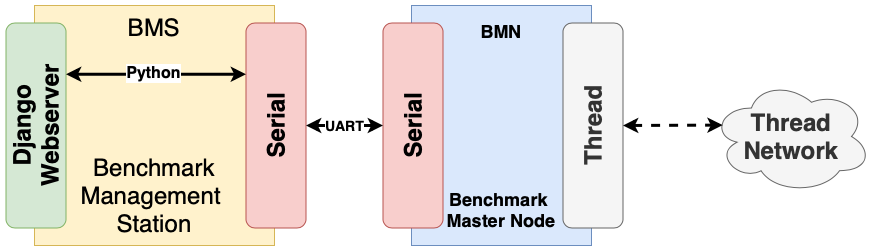
\includegraphics[width=1.0\textwidth]{Thread-Konzept.png}
	\caption{Konzept OpenThread Framework}\label{fig:ThreadKonzept}
\end{figure}


\subsubsection{Zigbee}\label{subsubsection:Zigbee}
Das Zigbee Test Mesh Netzwerk wird mithilfe der \textit{nRF SDK for Thread and Zigbee} eingerichtet und für die Messungen vorbereitet. Der BMN wird dabei als Zigbee Coordinator und gleichzeitig als Zigbee Router eingesetzt. Die BSN können wieder als Router oder aber als Zigbee End Device betrieben werden.

\newpage
\subsection{Steuer und Auswertesoftware}\label{subsec:SteuerundAuswertesoftware}
Die Steuerung des Testframeworks erfolgt über eine Weboberfläche. Diese wird von der BMS mittels WLAN auf den Benutzergeräten zur Anzeige gebracht. Als Webserver dient das Python-Framework \textit{Django}. Zur Steuerung der Benchmarks dienen Schrittketten, welche mit der Firmware auf dem BMN kommunizieren. Als letzter Schritt eines Benchmarks werden die Ergebnisse geloggt, nachbearbeitet und wiederum zur Anzeige gebracht.

Die Abbildung \ref{fig:EntwurfWebserver} stellt ein erstes Konzept dar, wie der Webserver für das P2P Test Framework aussehen kann. Die vom BMN ersichtlichen BSN werden aufgelistet und es können verschiedene  Aktionen durchgeführt werden. Mit Reitern soll auf verschiedene Seiten gewechselt werden auf welchen wiederum Resultate oder Logs der Kommunikation ersichtlich sein sollen.

\begin{figure}[H]
	\centering
	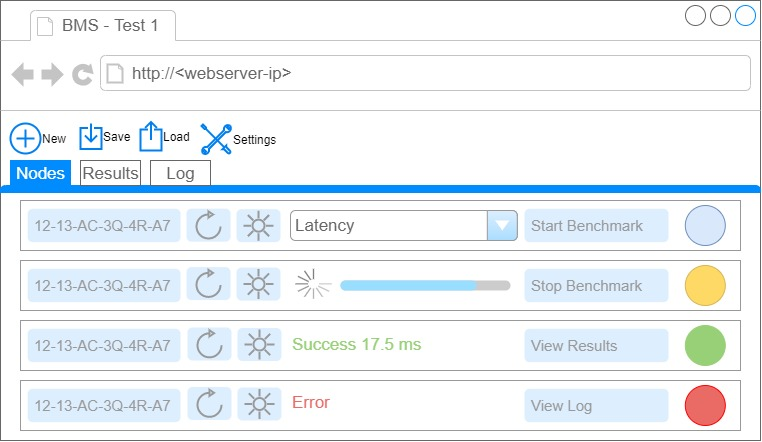
\includegraphics[width=1.0\textwidth]{Web_Mochup_BMS.jpg}
	\caption{Entwurf Webserver}\label{fig:EntwurfWebserver}
\end{figure}

